\documentclass[11pt,ngerman,a4paper]{article}
%Gummi|061|=)
\usepackage{amsmath}
\usepackage{a4wide}
\usepackage{url}
\usepackage{amsthm}
\usepackage{amsbsy}
\usepackage{amssymb}
\usepackage[utf8]{inputenc}
\usepackage{rotating} 
\usepackage{here}
\usepackage{graphicx}
\usepackage{paralist}
\usepackage{selinput}
\usepackage[separate-uncertainty=true]{siunitx}
\usepackage{booktabs}
\sisetup{}
\SelectInputMappings{%
adieresis={ä},
germandbls={ß},
}
\title{\textbf{Versuch V703: Geiger-Müller-Zählrohr}}
\author{Martin Bieker\\
		Julian Surmann\\
		\\
		Durchgef\"{u}hrt am 27.05.2014\\
		TU Dortmund}
\date{}
\usepackage{graphicx}
\begin{document}
\renewcommand\tablename{Tabelle}
\renewcommand\figurename{Abbildung}
\maketitle
\thispagestyle{empty}
\newpage
\clearpage
\setcounter{page}{1}


\section{Einleitung}
Das Geiger-Müller-Zählrohr ist ein einfaches Messinstrument zur Messung der Intensität von ionisierender Strahlung. In diesem Versuch werden einige Kenndaten dieser Apparatur ermittelt.
\section{Theorie}
\subsection{Aufbau und Funktion} 
 Das Geiger-Müller-Zählrohr besteht aus einem Draht  mit Radius $r_a$, der sich in einem Metallzylinder mit Radius $r_k$ befindet (siehe Abb. \ref{abb1}). 
\begin{figure}[htp]
\centering
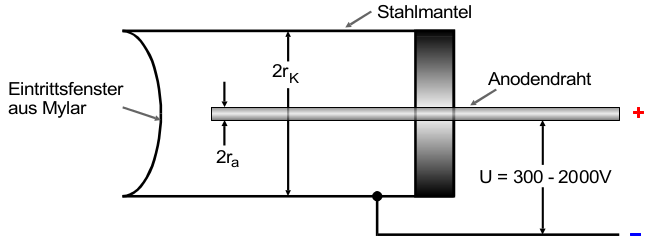
\includegraphics[scale=0.6]{abb1.png}
\caption{Aufbau eines Geiger-Müller-Zählrohrs. [1]}
\label{abb1}
\end{figure} 
Zwischen diesen Elementen wird eine elektrische Spannung von \SI{300}{\volt} bis \SI{2000}{\volt} angelegt. Auf diese Weise entsteht zwischen Anodendraht und Kathodenzylinder ein radial-symmetrisches Feld. Der Innenraum ist mit einem  Edelgasgemisch gefüllt. Da im Innenraum ein Unterdruck herrschen soll, ist das Zählrohr an den Enden verschlossen. An einer Seite befindet sich aber eine dünne Mylarfolie, damit  auch $\alpha$ und $\beta$-Teilchen in den Innenraum eindringen können.
 
 \noindent
 Wenn Strahlung in das Zählrohrvolumen eindringt, werden die Edelgasatome ionisiert. Da die Energie der Strahlung ein Vielfaches der Ionsierungsenergie ist, können mehrere Atome ionsiert werden, bis die Strahlung vollständig absorbiert ist. Die durch die Ionisierungsakte freigesetzten Elektronen werden durch das elektrische Feld  zum Anodendraht beschleunigt.
Die nach der ersten Ionisation ablaufenden Prozesse hängen sehr stark von der Zylinder anliegenden Spannung ab. In Abbildung \ref{abb2} wird die Anzahl der pro einfallendem Teilchen erzeugten Elektronen-Ionen-Paare als Funktion der am Zählrohr angelegten Spannung dargestellt.
\begin{figure}[htp]
\centering
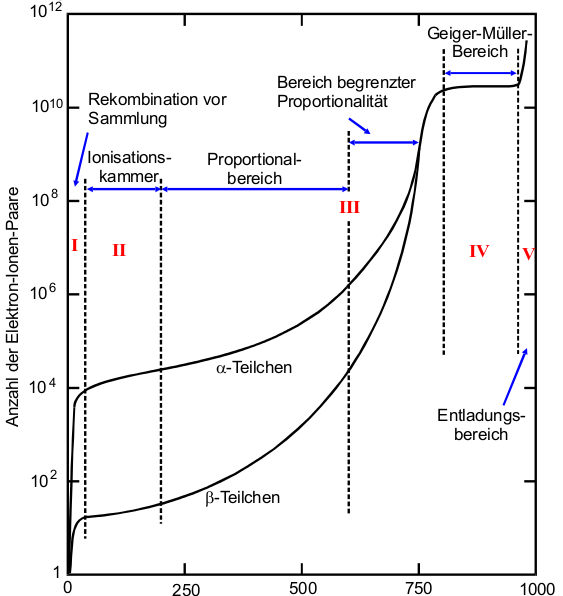
\includegraphics[scale=0.5]{abb2.png}
\caption{Anzahl der pro Teilchen erzeugten Ladungen als Funktion der Betriebsspannung.[1]}
\label{abb2}
\end{figure}
Ist das elektrische Feld nicht sehr stark, rekombinieren die Ionen bevor sie den Anodendraht erreichen. Dies entspricht Bereich I in der Abbildung. Wird die Spannung erhöht erreichen mehr Elektronen den Draht bevor sie rekombinieren können. In diesem Spannungsbereich (II in der Abbildung) wird das Zählrohr als Ionisationskammer betrieben. Bei weiterer Erhöhung der Spannung sind  die beschleunigten Elektronen auf Grund ihrer Energie in der Lage weitere Atome zu ionisieren. Es entsteht eine so genannte Townsend-Lawine. Es kann nun ein Ladungsimpuls gemessen werden, welcher von der Energie der einfallenden Strahlung abhängt. In diesem Bereich können mit dem Zählrohr sowohl die Intensität, als auch die Energie einer Strahlungsquelle gemessen werden. Daher wird die Apparatur in diesem Bereich als Proportionalitätszährohr bezeichnet. 
Steigt die Spannung weiter an, sind die Spannungsimpulse nicht mehr von der Teilchenenergie abhängig (Bereich IV). Bei der Ionisation durch die Elektronen entstehen auf Grund des starken elektrischen Feldes UV-Quanten. Da diese ungeladen sind, l\"osen sie auf ganzer Länge des Zählrohrs weitere Ionisationslawinen aus. In diesem Spannungsbereich wird ein Geiger-Müller-Zählrohr betrieben.
Bei weiterer Steigerung der Spannung wird die Apparatur durch Dauerentladungen zerstört.
\subsection{Charektersitik}
Die Anzahl der Ladungsimulse pro Zeit bei gegebener Quellenintensität in Abh\"angigkeit von der anliegenden Spannung wird als Charakteristik des Zählrohres bezeichnet. Diese ist beispielhaft in Abbildung \ref{abb3} dargestellt.
\begin{figure}[htp]
\centering
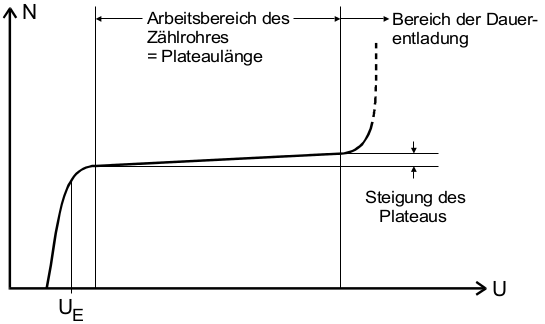
\includegraphics[scale=0.60]{abb3.png}
\caption{Charakterisktik eines Zählrohrs. [1]}
\label{abb3}
\end{figure}
Das in dieser Abbildung dargestellte Plateau ist der eigentliche Messbereich des Geiger-Müller-Zählrohrs. Die Länge und die Steigung des Plateaus sind wichtige Kennziffern für die Qualität der Apparatur.
 
\subsection{Totzeit und Nachtentladungen}

Die, bei den Ionisationsvorgängen entstehenden, positiven Edelgasionen haben im Vergleich zu den Elektronen eine sehr große Masse. Daher wandern diese nur langsam zur Kathode. Durch die im Zylinder vorherrschende positive Ladungsdichte schirmt das Feld indes Anodendrahts ab. Aus diesem Grund können für eine gewisse Zeit $T$ nach einem Impuls keine weiteren Teilchen erkannt werden. Dieser Effekt wird als Totzeit bezeichnet. Erst nachdem alle positiven Ionen neutralisiert wurden, erreichen die Ladungsimpulse ihre volle Stärke. Dieser Zeitraum heißt Erholungszeit $T_E$.

\noindent
Treffen die Edelgasionen auf den Kathodenzylinder lösen diese dort Elektronen aus der Metalloberfläche. Diese Elektronen können weitere Ionisations- und Entladungslawinen auslösen. Diese Nachentladungen verfälschen das Messergebnis, da dann bei einem Ladungsimpuls nicht unterschieden werden kann, ob dieser von einem Teilchen oder von einem Elektron aus dem Kathodenmaterial ausgelöst wurde. Um die Entstehung solcher Nachentladungen zu verhindern, wird dem Gas im Zählrohr eine geringe Menge eines Alkohols hinzugefügt. Diese relativ großen Moleküle nehmen die Energie der Ionen auf und wandeln diese in thermische Schwingungen um. Auf diese Weise können keine Elektronen aus der Metalloberfläche ausgelöst werden.
\section{Durchführung}
Der Versuch ist wie in Abbildung \ref{abb4} gezeigt aufgebaut.
\begin{figure}[htp]
\centering
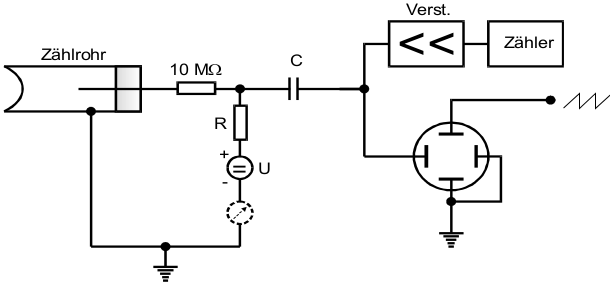
\includegraphics[scale=0.5]{abb4.png}
\caption{Schaltplan für Messungen am Geiger-Müller-Zählrohr. [1]}
\label{abb4}
\end{figure}
Das Zählrohr ist an eine variable Spannungsquelle angeschlossen. In einem hochohmigen Widerstand werden die Ladungsimpulse in Spannungsimpulse gewandelt und über einen Kondensator ausgekoppelt. Diese Impulse werden dann einerseits verstärkt und gezählt und andererseits mit einem Oszilloskop sichtbar gemacht.
\subsection{Aufnahme der Charakteristik}
Zur Aufnahme der Charakteristik wird ein $\beta$-Strahler vor dem Zählrohr angebracht und die Zählrate in Abhängigkeit von der Spannung gemessen. Dabei wird die Spannung von \SI{300}{\volt} bis \SI{700 }{\volt} in \SI{20}{\volt}-Schritten variiert. Damit der relative Fehler der Messung unter \SI{1}{\percent} bleibt, wird der Messzeitraum $\Delta t$
so gewählt, dass die Anzahl der gezählten Ereignisse
\[
N \geq \num{10000}
\]
ist. Zusätzlich wird mit einem Strommessgerät der durch das Zählrohr fließende Strom gemessen, um später die pro Teilchen freigesetzte Ladungsmenge zu bestimmen. 
\subsection{Oszillographische Messungen}
Zunächst sollen die Nachentladungen am Oszilloskop sichtbar gemacht werden. Dazu wird zunächst die Intensität der $\beta$-Quelle soweit gesenkt, dass die Wahrscheinlichkeit für zwei direkt aufeinander folgende Teilchen vernachlässigbar klein ist. Danach wird das Zählrohr einmal mit einer Spannung betrieben bei der Nachtentladungen unwahrscheinlich sind. Danach wird die Zählrohrspannung auf ihr Maximum von \SI{700}{\volt} erhöht.

\noindent
Danach soll die Totzeit und die Erholungszeit mit Hilfe des Oszilloskops bestimmt werden. Dazu wird eine hohe Stahlintensität gewählt. Es ergibt sich ein Oszillogramm wie in Abbildung \ref{abb5}.
\begin{figure}[htp]
\centering
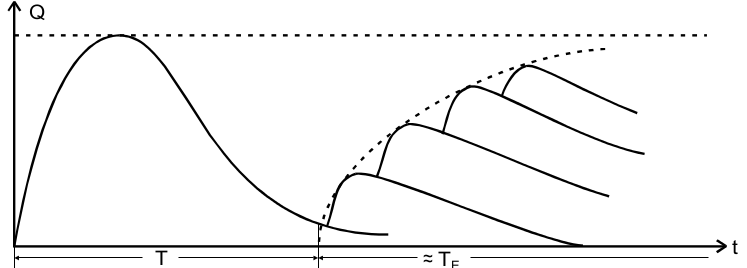
\includegraphics[scale=0.55]{abb5.png}
\caption{Schematische Darstellung eines Oszilogramms zur Bestimmung von Tot- und Erhohlungszeit. [1]}
\label{abb5}
\end{figure}
Aus diesem können Totzeit und die Erholungszeit grob abgelesen werden.
\subsection{Bestimmung der Totzeit mit der Zwei-Quellen-Methode}
Zur Bestimmung der Totzeit mit der Zwei-Quellen-Methode wird zunächst die Zählrate mit einer Quelle $N_1$ bestimmt. Danach wird eine zweite Quelle in den Versuchsaufbau eingebracht und die Zählrate beider Quellen $N_{1+2}$ ermittelt. Im Anschluss wird die erste Quelle entfernt und die Zählrate nur in Anwesenheit der zweiten Quelle $N_2$ gemessen. Die Totzeit $T$ ist dann durch 
\[
T \approx \frac{N_1 + N_2 - N_{1+2}}{2N_1N_2}
\]
gegeben.
 
\section{Auswertung}
Alle Fehler wurden mit python uncertainties errechnet.
\subsection{Aufnahme der Charakteristik}
Die gemessenen und errechneten Werte sind der Tabelle 1 zu entnehmen. Gemessen wurde die Zählrate bei einer Spannung von $\SI{300}{\volt}$ bis $\SI{700}{\volt}$.


\begin{table}[H]
\centering
\begin{tabular}{SSSSS}
\toprule
{U[V]} &{ N} &{ t[s]} &{ $I\left[\frac{1}{s}\right]$} &{ $\sigma_{I,rel}$[\%] }\\
\midrule
300.0 & 0.0 & 100.0 & 0 & nan\\
320.0 & 13617.0 & 250.0 & 54.5+-0.5 & 0.86\\
340.0 & 11192.0 & 200.0 & 56.0+-0.5 & 0.95\\
360.0 & 11231.0 & 200.0 & 56.2+-0.5 & 0.94\\
380.0 & 11601.0 & 200.0 & 58.0+-0.5 & 0.93\\
400.0 & 11410.0 & 200.0 & 57.0+-0.5 & 0.94\\
420.0 & 11459.0 & 200.0 & 57.3+-0.5 & 0.93\\
440.0 & 11496.0 & 200.0 & 57.5+-0.5 & 0.93\\
460.0 & 11433.0 & 200.0 & 57.2+-0.5 & 0.94\\
480.0 & 11379.0 & 200.0 & 56.9+-0.5 & 0.94\\
500.0 & 11457.0 & 200.0 & 57.3+-0.5 & 0.93\\
520.0 & 11437.0 & 200.0 & 57.2+-0.5 & 0.94\\
540.0 & 11376.0 & 200.0 & 56.9+-0.5 & 0.94\\
560.0 & 11564.0 & 200.0 & 57.8+-0.5 & 0.93\\
580.0 & 11620.0 & 200.0 & 58.1+-0.5 & 0.93\\
600.0 & 11333.0 & 200.0 & 56.7+-0.5 & 0.94\\
620.0 & 11382.0 & 200.0 & 56.9+-0.5 & 0.94\\
640.0 & 11449.0 & 200.0 & 57.2+-0.5 & 0.93\\
660.0 & 11414.0 & 200.0 & 57.1+-0.5 & 0.94\\
680.0 & 11507.0 & 200.0 & 57.5+-0.5 & 0.93\\
700.0 & 11642.0 & 200.0 & 58.2+-0.5 & 0.93\\
\bottomrule
\end{tabular}
\label{teil1}
\caption{Messdaten und Fehlerangabe}
\end{table}
\noindent
Die gemessene Charakteristik ist in Abbildung 6 zu sehen.
\begin{figure}[H]
\centering
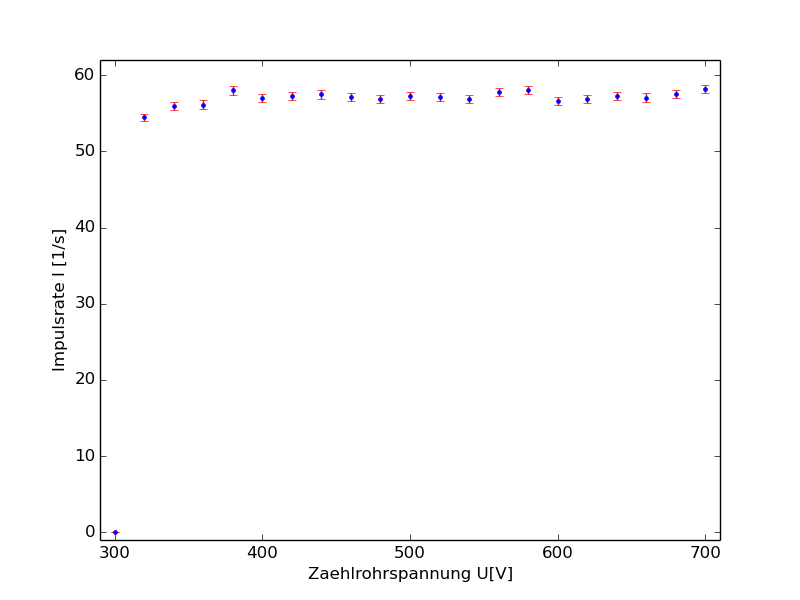
\includegraphics[scale=0.8]{plot1.png}
\label{plot1}
\caption{Messwerte}
\end{figure}
\noindent
An diesem Plot lässt sich ablesen, dass sich das Plateaus zwischen $\SI{340}{\volt}$ und $\SI{700}{\volt}$ befindet. Im Bereich des Plateaus wird nun eine lineare Regression durchgeführt. Diese ist in Abbildung 7 gezeigt.
\begin{figure}[H]
\centering
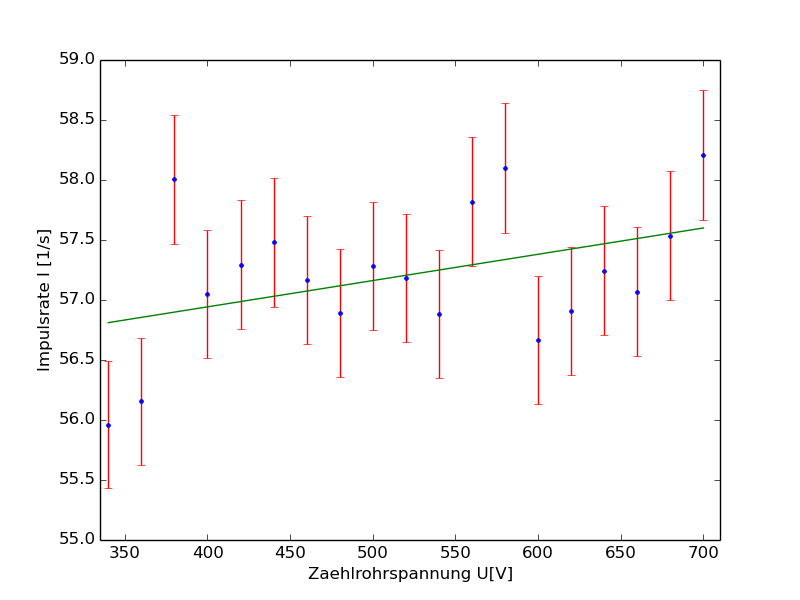
\includegraphics[scale=0.8]{plot2.png}
\label{plot2}
\caption{Lineare Regression}
\end{figure}
Als Regressionsgerade ergibt sich
\[
I(U) = \SI{0.0022\pm0.0011}{\per\volt\per\second} \cdot U + \SI{56.1\pm0.6}{\per\second}.
\]
Um die Steigung des Plateaus in \% pro $\SI{100}{\volt}$ zu berechnen, sind folgende ermittelte Werte benötigt:
\begin{itemize}
\item $\Delta U = \SI{360}{\volt}$
\item $I(340) = (56.8\pm0.7) \, \frac{1}{s}$
\item $I(700) = (57.6\pm1.0) \, \frac{1}{s}$
\end{itemize}
Damit ergibt sich die Steigung zu
\[
m_I = (0.46\pm0.23) \, \frac{\%}{100\, V}.
\]
\subsection{Zeitlicher Abstand zwischen Primär- und Nachentladungsimpuls}
Es werden am Oszilloskop die Werte
\begin{itemize}
\item $\SI{195+-1}{\micro\second}$
\item $\SI{163+-1}{\micro\second}$
\end{itemize}
abgelesen.
\subsection{Oszillographische Messung der Totzeit}
Die Totzeit wurde am Oszillographen abgelesen:
\[
T_{t} = \SI{124+-30}{\micro\second}.
\]
Die Erholungszeit konnte nur grob abgeschätzt werden. Es ergab sich
\[
T_E \approx \SI{467+-30}{\micro\second}.
\]
\subsection{Bestimmung der Totzeit mit der Zwei-Quellen-Methode}
Die gemessenen Werte der Zwei-Quellen-Methode sind in Tabelle 2 eingetragen.

\begin{table}[H]
\centering
\begin{tabular}{SSSSS}
\toprule
{Quelle} & {N} &{ t[s]} &{ $I\left[\frac{1}{s}\right]$} &{ $\sigma_{I,rel}$[\%] }\\
\midrule
{$N_1$} & 17483.0 & 200.0 & 87.4+-0.7 & 0.76\\
{$N_{1+2}$}& 20229.0 & 200.0 & 101.1+-0.7 & 0.70\\
{$N_2$} & 13280.0 & 1000.0 & 13.28+-0.12 & 0.87\\
\bottomrule
\end{tabular}
\label{blabla2}
\caption{Zweiquellenmethode}
\end{table}

\noindent
Als Wert für die Totzeit ergibt sich
\[
T_{t} = \SI{-0.0002+-0.0004}{\second}.
\]
Dieser Wert ist negativ, weil die gemeinsame Messung der Quellen eine höhere Intensität ergab als beide Einzelmessungen addiert. Im Rahmen der Unsicherheiten ist ein positiver Wert jedoch generell möglich. Der hier gemessene Wert hat jedoch keine Aussagekraft.
\subsection{Messung der pro Teilchen freigesetzten Ladungsmenge}
Die Messwerte, die zur Bestimmung der Ladung nötig sind, sowie die Ergebnisse sind in Tabelle 3 abgebildet.

\begin{table}[H]
\centering
\begin{tabular}{ccccccc}
\toprule
{U[V]} &{$ I[\mu A]$} &{ N} &{ t[s]} &{ $I\left[\frac{1}{s}\right]$} & $\sigma_{I,rel} [\%]$ &$ Q[10^{-7}C]$ \\
\midrule
320.0 & $0.05\pm0.05$ & 13617.0 & 250.0 & $54.5\pm0.5$ & 0.86 & $2.3\pm2.3$\\
340.0 & $0.05\pm0.05$ & 11192.0 & 200.0 & $56.0\pm0.5$ & 0.95 & $1.8\pm1.8$\\
360.0 & $0.10\pm0.05$ & 11231.0 & 200.0 & $56.2\pm0.5$ & 0.94 & $3.6\pm1.8$\\
380.0 & $0.15\pm0.05$ & 11601.0 & 200.0 & $58.0\pm0.5$ & 0.93 & $5.2\pm1.7$\\
400.0 & $0.17\pm0.05$ & 11410.0 & 200.0 & $57.0\pm0.5$ & 0.94 & $6.0\pm1.8$\\
420.0 & $0.19\pm0.05$ & 11459.0 & 200.0 & $57.3\pm0.5$ & 0.93 & $6.6\pm1.7$\\
440.0 & $0.20\pm0.05$ & 11496.0 & 200.0 & $57.5\pm0.5$ & 0.93 & $7.0\pm1.7$\\
460.0 & $0.20\pm0.05$ & 11433.0 & 200.0 & $57.2\pm0.5$ & 0.94 & $7.0\pm1.8$\\
480.0 & $0.20\pm0.05$ & 11379.0 & 200.0 & $56.9\pm0.5$ & 0.94 & $7.0\pm1.8$\\
500.0 & $0.22\pm0.05$ & 11457.0 & 200.0 & $57.3\pm0.5$ & 0.93 & $7.7\pm1.7$\\
520.0 & $0.23\pm0.05$ & 11437.0 & 200.0 & $57.2\pm0.5$ & 0.94 & $8.0\pm1.8$\\
540.0 & $0.24\pm0.05$ & 11376.0 & 200.0 & $56.9\pm0.5$ & 0.94 & $8.4\pm1.8$\\
560.0 & $0.25\pm0.05$ & 11564.0 & 200.0 & $57.8\pm0.5$ & 0.93 & $8.6\pm1.7$\\
580.0 & $0.30\pm0.05$ & 11620.0 & 200.0 & $58.1\pm0.5$ & 0.93 & $1.03\pm0.17$\\
600.0 & $0.35\pm0.05$ & 11333.0 & 200.0 & $56.7\pm0.5$ & 0.94 & $1.24\pm0.18$\\
620.0 & $0.40\pm0.05$ & 11382.0 & 200.0 & $56.9\pm0.5$ & 0.94 & $1.41\pm0.18$\\
640.0 & $0.40\pm0.05$ & 11449.0 & 200.0 & $57.2\pm0.5$ & 0.93 & $1.40\pm0.18$\\
660.0 & $0.40\pm0.05$ & 11414.0 & 200.0 & $57.1\pm0.5$ & 0.94 & $1.40\pm0.18$\\
680.0 & $0.45\pm0.05$ & 11507.0 & 200.0 & $57.5\pm0.5$ & 0.93 & $1.56\pm0.17$\\
700.0 & $0.50\pm0.05$ & 11642.0 & 200.0 & $58.2\pm0.5$ & 0.93 & $1.72\pm0.17$\\
\bottomrule
\end{tabular}
\label{tab3}
\caption{Messung der pro Teilchen freigesetzten Ladungsmenge}
\end{table}
Der gemessene Strom in Abhängigkeit von der Betriebsspannung ist in Abbildung 8 zu sehen.
\begin{figure}[H]
\centering
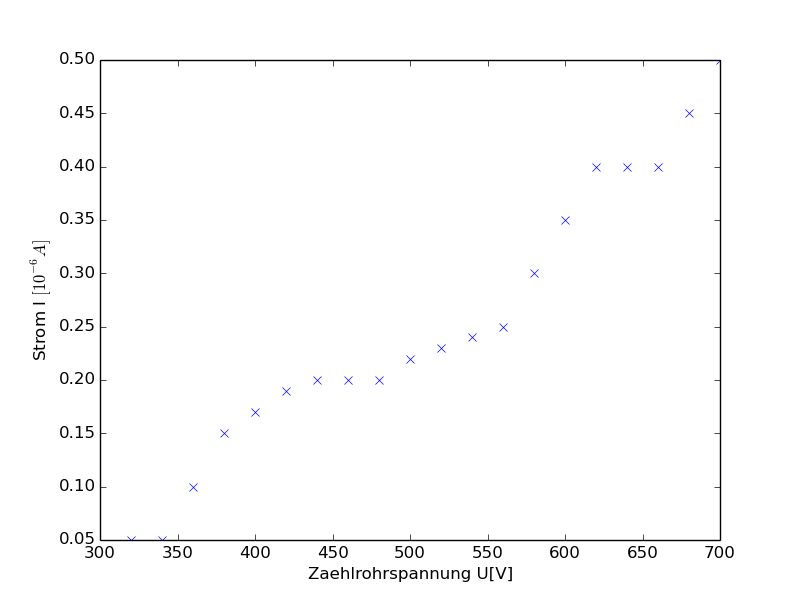
\includegraphics[scale=0.6]{plot3.png}
\caption{Messwerte}
\label{plot3}
\end{figure}
\noindent
Diese Messwerte sind so fehlerbehaftet, dass eine weitere Auswertung zwecklos ist. Es ergäbe sich ein linearer Zusammenhang.
\section{Diskussion}
Auffällig ist die hohe statistische Abweichung der Messwerte. Die für die lineare Regression verwendeten Werte weisen hohe Schwankungen auf.
Alle vom Oszilloskop abgelesenen Werte sind sehr ungenau. Sie konnten nur geschätzt werden. Die Messung mit der Zwei-Quellen-Methode hat nicht funktioniert. Einen Grund hierfür könnte die geringe Aktivität der radioaktiven Proben sein, da so kaum Energie-Emissionen während der Totzeiten auftreten. Die letzte Messung war leider mit einem sehr großen Fehler behaftet, da die Empfindlichkeit des Amperemeters kaum geeignet war.

\section{Quellen}
\begin{enumerate}[{[}1{]}]
\item Entnommen der Praktikumsanleitung \textit{} der TU Dortmund. \\
Download am 01.06.14 unter:\\
 \url{http://129.217.224.2/HOMEPAGE/PHYSIKER/BACHELOR/AP/SKRIPT/V703.pdf}
\end{enumerate}

\section{Anhang}
\begin{itemize}
\item Auszug aus dem Messheft
\end{itemize}
\end{document}
